\section{Numerical Evaluation}
\label{sec:experiments}

We evaluate the PEG numerically across four experiments. Each isolates one
distinct question that the framework raises. \cref{tab:experiments-overview}
summarises what each one asks, what it controls for, and what it answers.

\begin{table}[t]
\centering
\caption{Overview of the four numerical experiments.}
\label{tab:experiments-overview}
\small
\begin{tabular}{lp{1.7cm}p{2.5cm}p{1.8cm}}
\toprule
 & Question & Setup & Finding \\
\midrule
C1 & Symmetric equilibrium? & 2 equal-size groups, full $\boldsymbol{\eps}$-grid sweep & 8 NEs, all asymmetric (\cref{fig:C1}) \\
C2 & Effect of size asymmetry & 2 groups, size ratio $r \in [0.1, 10]$ & Minority plays low $\eps$, majority absorbs $A$ (\cref{fig:C2}) \\
C4 & How bad under coordination? & $n{=}5$, target $\eps_t{=}32$, coalition of size $k$ & $A_t$ monotone in $k$; $+65\%$ at $k{=}4$ (\cref{fig:C4}) \\
C5 & Where does the externality come from? & 2-group, vary $\eps_O$ and proportion at fixed $\eps_T$ & $A_t$ monotone in $\eps_O$, crossover at $\eps_O{=}\eps_T$ (\cref{fig:C5}) \\
\bottomrule
\end{tabular}
\end{table}

\subsection{Common setup}
\label{sec:setup}

All experiments are analytical---no model training---and follow the same
mechanism-solver and advantage-computation pipeline.

\paragraph{Mechanism solver.} For each action profile $\boldsymbol{\eps}$ we
compute the mechanism solution $(\sigma, p_1,\dots,p_n)$ by bisecting on
$\sigma$ until the batch-size constraint (C2) is met, with each per-group
sampling rate chosen to make the (C1) RDP constraint
bind~\cite{mironov2017renyi}. Profiles in which any $p_i$ falls below a small
participation threshold are flagged as infeasible
(\cref{ass:participation}). We then compute each realised $A_i$ exactly from
the privacy profile of the $I$-fold $(p_i, \sigma)$-subsampled Gaussian using
PLD accounting~\cite{google-dp-accounting}, recovering the formula
of~\eqref{eq:adv}.

\paragraph{Action space.} Unless stated, the action space is the
log-spaced grid $\mathcal{A}_K \subset [0.5, 64]$ with $K = 22$ points,
$\delta = 10^{-12}$. We verified on a refined grid ($K = 44$) that the NEs
reported are stable to grid refinement, so we report them as representative
of the continuous-action equilibrium.

\paragraph{Scenarios.} Unless stated, all experiments use $n$ symmetric
groups of $|G_g| = 5000$ samples each, expected batch size $E_b = 128$,
$5$ epochs of training, $B_i = C_i = 1$, and $V(\sigma) = 1/(1+\sigma^2)$.
These choices broadly mirror the empirical iDP scenarios of
\cite{kaiser2026your, boenisch2023have}.

\begin{table}[t]
\centering
\caption{Pure Nash equilibria of the symmetric 2-player PEG on the log-spaced action grid $\mathcal{A}_K = $ 22 points in $[0.5, 64]$, $|G_1|=|G_2|=5000$, $E_b=128$, $5$ epochs, $\delta=10^{-12}$, $B_i = C_i = 1$, $V(\sigma) = 1/(1+\sigma^2)$. Social optimum is the feasible action profile maximising $u_1+u_2$.}
\label{tab:NE}
\begin{tabular}{lcccc}
\toprule
 & $(\varepsilon_1^*, \varepsilon_2^*)$ & $A_1$ & $A_2$ & $\sigma$ \\
\midrule
NE$_{1}$ & $(0.79, 5.04)$ & 0.001 & 0.202 & 1.160 \\
NE$_{2}$ & $(1.26, 6.35)$ & 0.002 & 0.232 & 1.028 \\
NE$_{3}$ & $(1.59, 8.00)$ & 0.002 & 0.266 & 0.929 \\
NE$_{4}$ & $(2.52, 3.17)$ & 0.081 & 0.120 & 1.186 \\
NE$_{5}$ & $(3.17, 2.52)$ & 0.120 & 0.081 & 1.186 \\
NE$_{6}$ & $(5.04, 0.79)$ & 0.202 & 0.001 & 1.160 \\
NE$_{7}$ & $(6.35, 1.26)$ & 0.232 & 0.002 & 1.028 \\
NE$_{8}$ & $(8.00, 1.59)$ & 0.266 & 0.002 & 0.929 \\
social opt & $(5.04, 25.40)$ & 0.007 & 0.535 & 0.590 \\
\bottomrule
\end{tabular}
\end{table}

% =====================================================================
\subsection{C1 --- Does the symmetric 2-player game admit a symmetric NE?}
\label{sec:C1}

\paragraph{Setup.} Two players, equal group sizes
$|G_1|=|G_2|=5000$. Sweep both players' $\eps$ over the dense
log-spaced grid; brute-force search for all pure NEs.

\paragraph{Finding.} \emph{No.} The BR correspondences cross at \emph{eight}
points, all off the diagonal (\cref{fig:C1}, centre; \cref{tab:NE}). The
pairs $(0.79, 5.04), (1.26, 6.35), (1.59, 8.00), (2.52, 3.17)$ and their
swaps are pure NEs; the realised $A$ at these equilibria ranges from
$(A_1, A_2) = (0.001, 0.202)$ at the most asymmetric pair down to
$(0.081, 0.120)$ at the closest-to-symmetric pair. No NE sits on the
diagonal.

\paragraph{Implication.} Even when the game is fully symmetric in players,
group sizes, and weights, \emph{the equilibrium breaks symmetry}. The
intuition is in \cref{lem:externality}: at any symmetric profile both
players face an identical incentive to deviate downward in $\eps$; only an
off-diagonal profile resolves the deadlock by having one player carry $V$
and the other carry low $A$.

\begin{figure*}[!t]
\centering
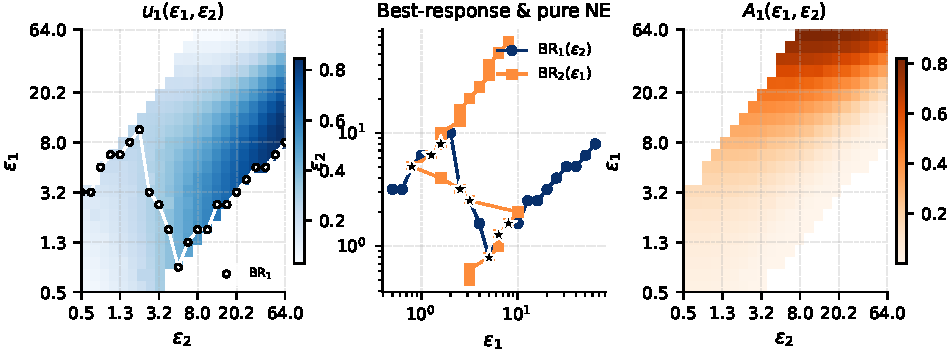
\includegraphics[width=\linewidth]{figures/fig_C1_payoff.pdf}
\caption{\textbf{C1.} 2-player payoff surface $u_1(\eps_1,\eps_2)$ (left),
best-response correspondences with pure NEs as black stars (centre), and
realised MIA advantage $A_1$ (right). All eight pure NEs lie off the
diagonal.}
\label{fig:C1}
\end{figure*}

% =====================================================================
\subsection{C2 --- Who absorbs the externality when groups differ in size?}
\label{sec:C2}

\paragraph{Setup.} Two players, dataset size ratio $|G_1|/|G_2| \in
\{0.1, 0.25, 0.5, 1, 2, 4, 10\}$ at fixed total $M=10000$, fixed batch
$E_b{=}128$. Full grid sweep at each ratio; for each ratio we report the
pure NE with the largest asymmetry in realised $A$.

\paragraph{Finding.} \emph{The minority always plays the lower $\eps$ and
absorbs less of the realised vulnerability.} \cref{fig:C2}: for $r < 1$
(group 1 smaller) the equilibrium has $\eps_1^* \in [1.5, 3]$ and
$\eps_2^* \approx 10$, giving $A_1^* < 0.01$ and $A_2^* \in [0.24, 0.32]$.
For $r > 1$ the pattern flips by symmetry. At $r{=}1$ the C1 NE structure
is recovered.

\paragraph{Implication.} The externality has a \emph{group-size sign}.
Because (C2) enforces a fixed expected batch, a small-group player who
demands strong privacy contributes little to the batch and forces the
large-group player's $p$ upward; the latter therefore carries the realised
$A$. This is a privacy analogue of a free-riding result: small groups
gain disproportionately from the externality and large groups pay
disproportionately for it.

\begin{figure*}[!t]
\centering
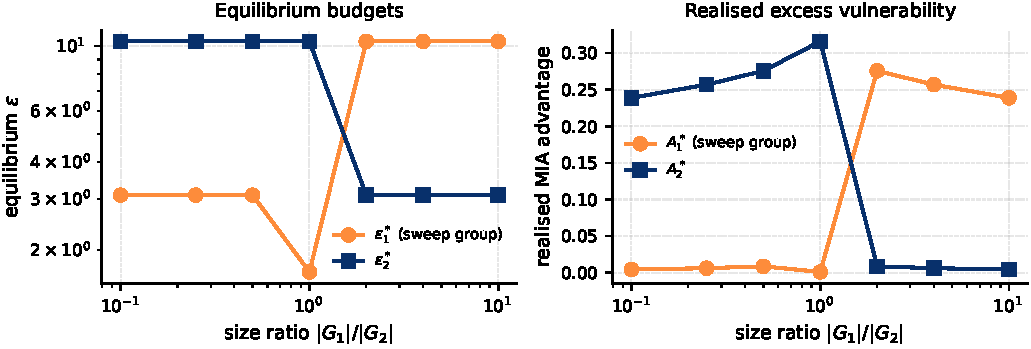
\includegraphics[width=\linewidth]{figures/fig_C2_asymmetric.pdf}
\caption{\textbf{C2.} Equilibrium budget (left) and realised MIA advantage
(right) as a function of dataset size ratio $|G_1|/|G_2|$. The minority
group's $\eps^*$ is always lower than the majority's, and its realised
$A^*$ correspondingly smaller. The flip at $r{=}1$ is the boundary at
which the minority/majority labels exchange.}
\label{fig:C2}
\end{figure*}

% =====================================================================
\subsection{C4 --- How severe does the attack get under coordination?}
\label{sec:C4}

\paragraph{Setup.} Five symmetric players, all with $|G_g|=5000$. Player $0$
is the target with $\eps_t = 32$. The remaining $n-1=4$ players are
partitioned into a coalition $C$ of size $k$ (varied) and a non-coalition
fixed at $\eps = 32$. The coalition picks the action that maximises $A_t$
(Stackelberg leader, $\lambda \to \infty$).

\paragraph{Finding.} \emph{$A_t$ is monotone-increasing in $k$, with a
non-trivial optimal coalition budget.} \cref{fig:C4}: baseline $A_t = 0.442$
(no coalition) rises to $0.483$ at $k{=}1$, $0.531$ at $k{=}2$, $0.607$ at
$k{=}3$, and $0.728$ at $k{=}4$. The optimum coalition budget is
$\eps^\star \approx 6.8$ for $k \in \{1,2,3\}$ and drops to $\eps^\star
\approx 3.2$ at $k = 4$: the participation-preserving minimum decreases
as the coalition grows because more colluders can absorb the same
externality between them while keeping each $p_i > 0$.

\paragraph{Implication.} The budget-manipulation attack of
\citet{kaiser2026your} is the rational best response of a coordinated
subset of data holders in the PEG. The empirical $62\%$ attack-success
rate reported in their work corresponds to the same equilibrium our
framework predicts; \cref{fig:C4} traces its severity as a function of the
coordinated coalition's size.

\begin{figure}[!t]
\centering
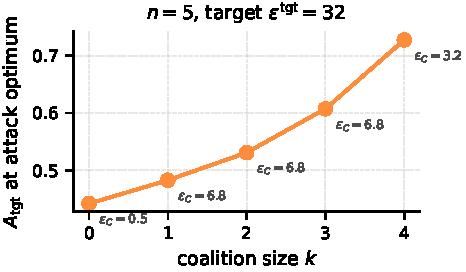
\includegraphics[width=\linewidth]{figures/fig_C4_coalition.pdf}
\caption{\textbf{C4.} Target's realised MIA advantage as a function of
coalition size $k$, with the coalition playing its target-maximising joint
action. Annotations show the optimal coalition budget $\eps^\star$ at each
$k$.}
\label{fig:C4}
\end{figure}

% =====================================================================
\subsection{C5 --- What is the functional form of the externality?}
\label{sec:C5}

\paragraph{Setup.} Two groups, target with budget $\eps_T \in \{4, 16\}$
fixed, others' budget $\eps_O$ swept over the log-spaced grid. The other
group's proportion of the total dataset is varied over
$\{0.2, 0.4, 0.6, 0.8\}$ at fixed total size $M = 10000$. This isolates the
target's vulnerability as a pure function of (a) what the others choose
and (b) how many of them there are.

\paragraph{Finding.} \emph{$A_t$ is monotone-decreasing in $\eps_O$; the
proportion-curves cross exactly at $\eps_O = \eps_T$.} \cref{fig:C5}: at
$\eps_T = 4$, $A_t$ ranges from $\approx 0.20$ (others at $\eps_O = 0.5$)
to $\approx 0$ (others at $\eps_O = 64$). At $\eps_T = 16$, the range is
$0.55$ down to $\approx 0.05$. For $\eps_O < \eps_T$ a larger proportion
of others raises $A_t$; for $\eps_O > \eps_T$ a larger proportion of
others lowers $A_t$. The crossover at $\eps_O = \eps_T$ is the regime in
which the others' choice and the target's choice contribute identically
to $\sigma$.

\paragraph{Implication.} This isolates the externality as a pure mechanism
effect, independent of any strategic choice. The shape mirrors Figure~3 of
\citet{kaiser2026your}, who showed the same dependence empirically through
the iDP-SGD trade-off function. C5 confirms that the externality lemma
(\cref{lem:externality}) is not just empirically monotone but
\emph{quantitatively} so: each unit decrease in others' $\eps$ corresponds
to a smooth, predictable increase in the target's realised $A$.

\begin{figure*}[!t]
\centering
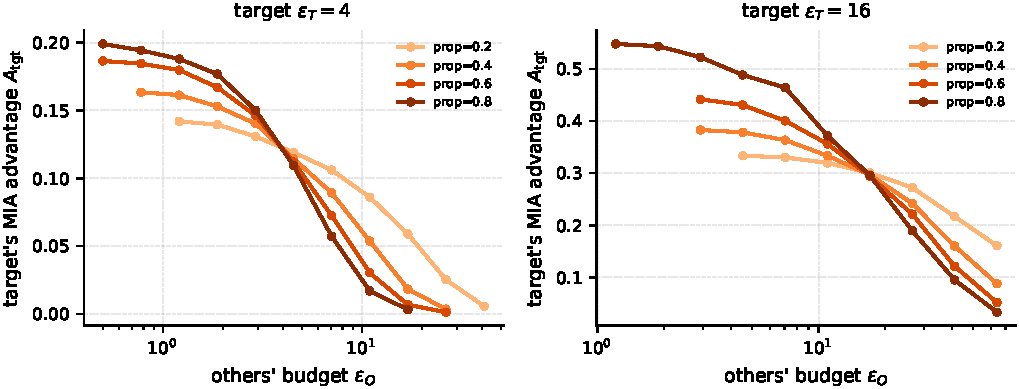
\includegraphics[width=\linewidth]{figures/fig_C5_surface.pdf}
\caption{\textbf{C5.} Target's realised MIA advantage as a function of the
other group's budget $\eps_O$ and proportion, at two fixed target budgets
$\eps_T \in \{4, 16\}$. The curves cross at $\eps_O = \eps_T$. Below
crossover, larger proportions raise $A_t$; above crossover, larger
proportions lower it.}
\label{fig:C5}
\end{figure*}
